\documentclass{article}
\usepackage{amsmath}
\usepackage{amssymb}
\usepackage{graphicx}
\usepackage{float}
\usepackage[margin=1cm,footskip=0.25cm]{geometry}
\usepackage{tikz}
\usetikzlibrary{shapes.geometric, positioning, arrows.meta, automata}

\begin{document}
\begin{center}
    \textbf{\LARGE Theoretische Informatik}
\end{center}

\section*{Alphabete, Wörter und Sprachen}
\begin{minipage}[t]{0.45\textwidth}
    \subsection*{Alphabete}
    Ein \textbf{Alphabet} $\Sigma$ ist eine endliche, nichtleere Menge von Symbolen.
    
    \subsection*{Sprachen}
    Eine \textbf{Sprache} $L$ über einem Alphabet $\Sigma$ ist eine Menge von Wörtern, die aus Symbolen von $\Sigma$ bestehen. Eine Sprache kann endlich oder unendlich sein. Die leere Sprache wird mit $\emptyset$ bezeichnet.
\end{minipage}
\hfill
\begin{minipage}[t]{0.45\textwidth}
    \subsection*{Wörter}
    Ein \textbf{Wort} $w$ ist eine endliche Folge von Symbolen aus einem Alphabet $\Sigma$. Die Länge eines Wortes $w$ wird mit $|w|$ bezeichnet. Das leere Wort wird mit $\varepsilon$ dargestellt und hat die Länge 0.
    Die Menge aller Wörter über einem Alphabet $\Sigma$ wird mit $\Sigma^*$ bezeichnet (Kleenesche Hülle). 
\end{minipage}
\section*{Endliche Automaten}
\begin{minipage}[t]{0.45\textwidth}
    \subsection*{Deterministische endliche Automaten (DEA)}
    Ein DEA ist ein 5-Tupel $M = (Q, \Sigma, \delta, q_0, F)$, wobei:
    \begin{itemize}
        \item $Q$ eine endliche Menge von Zuständen ist,
        \item $\Sigma$ ein Alphabet ist,
        \item $\delta: Q \times \Sigma \to Q$ die Übergangsfunktion ist,
        \item $q_0 \in Q$ der Startzustand ist,
        \item $F \subseteq Q$ die Menge der Endzustände ist.
    \end{itemize}
    \textbf{Übergangsfunktion:} $\delta(q_0, a_1) = q_1$

    Ein Wort $w \in \Sigma^*$ wird akzeptiert, wenn es von $M$ verarbeitet wird und der Endzustand in $F$ liegt.
\end{minipage}
\hfill
\begin{minipage}[t]{0.45\textwidth}
    \subsection*{Nichtdeterministische endliche Automaten (NEA)}
    Ein NEA ist ähnlich aufgebaut, aber die  Übergangsfunktion $\delta$ kann mehrere Zustände für ein Symbol zurückgeben: 
    $\delta: Q \times \Sigma \to 2^Q$. Ein NEA akzeptiert ein Wort, wenn es mindestens einen Pfad gibt, der das Wort vollständig verarbeitet und in einem Endzustand endet.

    \begin{center}
        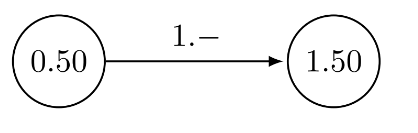
\includegraphics[scale=0.5]{images/ea.png}
    \end{center}
\end{minipage}

\vspace{0.5cm}

\section*{Kontextfreie Grammatiken}
\begin{minipage}[t]{0.45\textwidth}
    \subsection*{Definition}
    Eine \textbf{kontextfreie Grammatik} (KFG) ist ein 4-Tupel $G = (V, \Sigma, P, S)$, wobei:
    \begin{itemize}
        \item $V$ eine endliche Menge von Variablen ist,
        \item $\Sigma$ ein Alphabet ist (Terminale),
        \item $P$ eine endliche Menge von Produktionen ist,
        \item $S \in V$ das Startsymbol ist.
    \end{itemize}
    \subsection*{Produktionen}
    Eine Produktion hat die Form $A \to \alpha$, wobei $A \in V$ und $\alpha \in (V \cup \Sigma)^*$. Die Ableitung eines Wortes erfolgt durch wiederholtes Anwenden der Produktionen.
\end{minipage}
\hfill
\begin{minipage}[t]{0.45\textwidth}
    \subsection*{Ableitung}
    Ein Wort $w$ wird aus $G$ abgeleitet, wenn es durch eine endliche Folge von Produktionen aus dem Startsymbol $S$ entsteht. Die Menge aller Wörter, die aus $G$ abgeleitet werden können, bildet die Sprache $L(G)$ der Grammatik.
    \begin{center}
        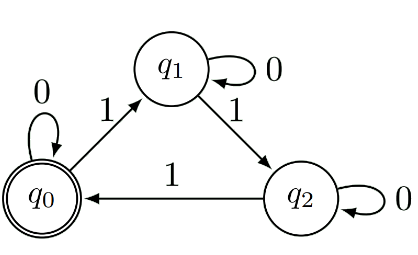
\includegraphics[scale=0.5]{images/kfg.png}
    \end{center}
\end{minipage}
\section*{Kellerautomaten (KA)}
\begin{minipage}[t]{0.45\textwidth}
    Ein \textbf{Kellerautomat} (Pushdown automata) (PDA) ist ein endlicher Automat, der zusätzlich einen Keller (Stack) hat. 
    Er kann Symbole auf den Stack legen und entfernen. Ein Kellerautomat wird durch ein 7-Tupel $M = (Q, \Sigma, \Gamma, \delta, q_0, Z_0, F)$ definiert:
    \begin{itemize}
        \item $Q$ eine endliche Menge von Zuständen,
        \item $\Sigma$ ein Eingabealphabet,
        \item $\Gamma$ ein Kelleralphabet,
        \item $\delta: Q \times \Sigma \times \Gamma \to 2^{Q \times \Gamma^*}$ die Übergangsfunktion,
        \item $q_0 \in Q$ der Startzustand,
        \item $Z_0 \in \Gamma$ das Startsymbol des Kellers,
        \item $F \subseteq Q$ die Menge der Endzustände.
    \end{itemize}
    \textbf{Übergangsfunktion:} $\delta(q_0, a_1, Z_0) = (q_1, Z_0 a_2)$
    \begin{enumerate}
        \item Ist im Zustand $q_0$ 
        \item wird das Symbol $a_1$ gelesen,
        \item wird das Symbol $Z_0$ vom Keller gepopt,
        \item wechselt der Automat in den Zustand $q_1$,
        \item und legt das Symbol $Z_0 a_2$ auf den Keller.
    \end{enumerate}
    
    Ein Kellerautomat akzeptiert ein Wort, wenn es in einem Endzustand endet und der Keller leer ist.
\end{minipage}
\hfill
\begin{minipage}[t]{0.45\textwidth}
    \begin{center}
        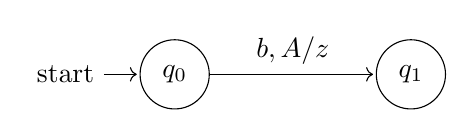
\begin{tikzpicture}[shorten >=1pt, node distance=3cm, on grid, auto]
            % Zustände
            \node[state, initial] (q0) {$q_0$};
            \node[state, right=of q0] (q1) {$q_1$};
            
            % Übergänge
            \path[->]
            % (q0) edge[loop above] node[align=left] {$a, Z_0/A Z_0$\\$a, A/AA$} ()
            (q0) edge[left] node[above] {$b, A/z$} (q1);
        \end{tikzpicture}
        \end{center}
        \textit{Legende: $b, A/z$ bedeutet: lese $b$ aus Wort, poppe $A$ vom Keller, pushe $z$ auf den Keller.}
        
        \section*{Vergleich der Typen}
        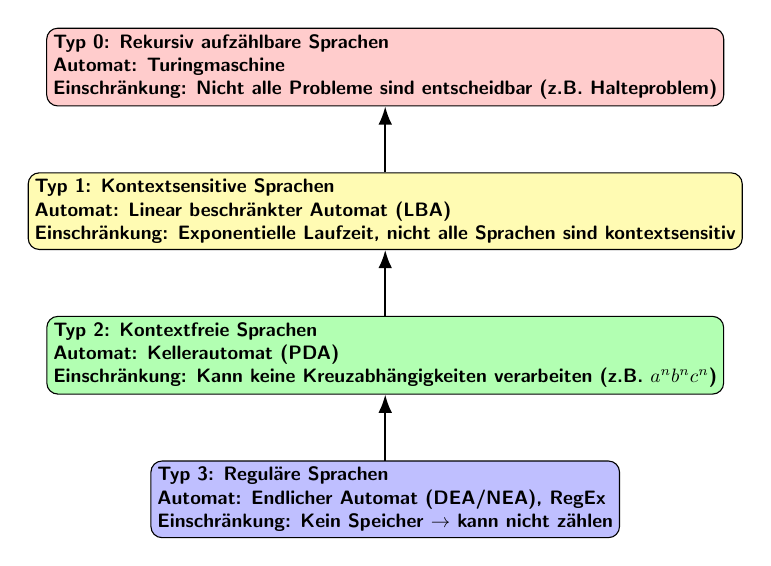
\begin{tikzpicture}[
          scale=0.7,
          transform shape,
          box/.style = {draw, rounded corners, minimum width=4.2cm, minimum height=1.2cm, align=left, font=\bfseries\sffamily, fill=gray!10},
          note/.style = {font=\small, align=left},
          level distance=1cm
         ]

        % Typ 0 - Turingmaschinen
        \node[box, fill=red!20] (type0) {
        Typ 0: Rekursiv aufzählbare Sprachen\\
        \textbf{Automat:} Turingmaschine\\
        \textbf{Einschränkung:} Nicht alle Probleme sind entscheidbar (z.B. Halteproblem)
        };
        
        % Typ 1 - Kontextsensitive Sprachen
        \node[box, below=1.2cm of type0, fill=yellow!30] (type1) {
        Typ 1: Kontextsensitive Sprachen\\
        \textbf{Automat:} Linear beschränkter Automat (LBA)\\
        \textbf{Einschränkung:} Exponentielle Laufzeit, nicht alle Sprachen sind kontextsensitiv
        };
        
        % Typ 2 - Kontextfreie Sprachen
        \node[box, below=1.2cm of type1, fill=green!30] (type2) {
        Typ 2: Kontextfreie Sprachen\\
        \textbf{Automat:} Kellerautomat (PDA)\\
        \textbf{Einschränkung:} Kann keine Kreuzabhängigkeiten verarbeiten (z.B. $a^n b^n c^n$)
        };
        
        % Typ 3 - Reguläre Sprachen
        \node[box, below=1.2cm of type2, fill=blue!25] (type3) {
        Typ 3: Reguläre Sprachen\\
        \textbf{Automat:} Endlicher Automat (DEA/NEA), RegEx\\
        \textbf{Einschränkung:} Kein Speicher $\rightarrow$ kann nicht zählen
        };
        
        % Pfeile (Enthalten)
        \draw[-{Latex}, thick] (type3.north) -- (type2.south);
        \draw[-{Latex}, thick] (type2.north) -- (type1.south);
        \draw[-{Latex}, thick] (type1.north) -- (type0.south);
        
        \end{tikzpicture}
\end{minipage}
\section*{Turingmaschinen}
\begin{minipage}[t]{0.45\textwidth}
    Eine \textbf{Turingmaschine} (TM) ist ein theoretisches Rechenmodell, das aus einem endlichen Steuerwerk, einem unendlichen Band und einem Lesekopf besteht. Sie kann Symbole auf dem Band lesen und schreiben sowie den Kopf bewegen.
    
    Eine Turingmaschine wird durch ein 7-Tupel $M = (Q, \Sigma, \Gamma, \delta, q_0, q_{reject}, q_{accept})$ definiert:
    \begin{itemize}
        \item $Q$ eine endliche Menge von Zuständen,
        \item $\Sigma$ ein Eingabealphabet (ohne das leere Symbol),
        \item $\Gamma$ ein Bandalphabet (enthält $\Sigma$ und das leere Symbol),
        \item $\delta: Q \times \Gamma \to Q \times \Gamma \times \{L, R, S\}$ die Übergangsfunktion,
        \item $q_0 \in Q$ der Startzustand,
        \item $q_{reject} \in Q$ der Ablehnungszustand,
        \item $q_{accept} \in Q$ der Akzeptierzustand.
    \end{itemize}

    \subsubsection*{Gödel-Nummerierung}
    \{Aktueller Zustand\}1\{Symbol auf dem Band\}1\{Nächster Zustand\}1\{Symbol schreiben\}1\{Richtung bewegen (R=00, L=0)\}11
\end{minipage}
\hfill
\begin{minipage}[t]{0.45\textwidth}
    \textbf{Übergangsfunktion:} $\delta(q_0, X) = (q_1, Y, R)$ bedeutet:
    \begin{enumerate}
        \item Im Zustand $q_0$ wird das Symbol $X$ gelesen,
        \item der Zustand wechselt zu $q_1$,
        \item das Symbol auf dem Band wird zu $Y$ geändert,
        \item der Lesekopf bewegt sich nach rechts (R).
    \end{enumerate}
    Eine Turingmaschine akzeptiert ein Wort, wenn sie in den Zustand $q_{accept}$ wechselt und das Band in einem akzeptierenden Zustand endet.
    \begin{center}
        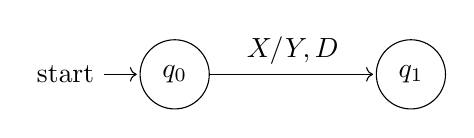
\begin{tikzpicture}[shorten >=1pt, node distance=3cm, on grid, auto]
            % States
            \node[state, initial] (q0) {$q_0$};
            \node[state, right=of q0] (q1) {$q_1$};
            
            % q0 loop
            \path[->]
            % (q0) edge[loop above] node[align=left] {$a, Z_0/A Z_0$\\$a, A/AA$} ()
            (q0) edge[left] node[above] {$X/Y,D$} (q1);
        \end{tikzpicture}
    \end{center}
    \textit{Legende: $x/y,D$ bedeutet: lese $x$, schreibe $y$ auf das Band, bewege den Kopf in Richtung $D$ (L für links, R für rechts, S für stehenbleiben).}
\end{minipage}

\section*{Berechenbarkeit}
\begin{minipage}[t]{0.45\textwidth}
    \subsection*{Entscheidbare Probleme}
    Ein Problem ist \textbf{entscheidbar}, wenn es eine Turingmaschine gibt, die für jede Eingabe in endlicher Zeit entscheidet, ob die Eingabe zur Sprache gehört oder nicht.
    Jede entscheidbare Sprache ist auch semi-entscheidbar.
    
    \subsection*{semi-entscheidbare Probleme}
    Ein Problem ist \textbf{semi-entscheidbar}, wenn es eine Turingmaschine gibt, die für jede Eingabe, die zur Sprache gehört, in endlicher Zeit akzeptiert, aber für Eingaben, die nicht zur Sprache gehören, möglicherweise nicht terminiert.

    \subsection*{Unentscheidbare Probleme}
    Ein Problem ist \textbf{unentscheidbar}, wenn es keine Turingmaschine gibt, die für alle Eingaben in endlicher Zeit entscheidet. Ein bekanntes Beispiel ist das Halteproblem.
\end{minipage}
\hfill
\begin{minipage}[t]{0.45\textwidth}
    \begin{center}
        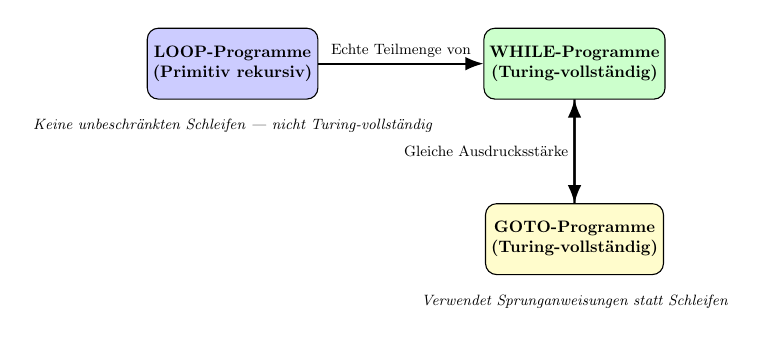
\begin{tikzpicture}[
        scale=0.6,
        transform shape,
        box/.style = {draw, rounded corners, minimum width=3.5cm, minimum height=1.5cm, align=center, font=\bfseries, fill=gray!10},
        arrow/.style = {-{Latex}, thick},
        note/.style = {font=\small\itshape}
        ]
    
        % Knoten
        \node[box, fill=blue!20] (loop) {LOOP-Programme\\(Primitiv rekursiv)};
        \node[box, right=3.5cm of loop, fill=green!20] (while) {WHILE-Programme\\(Turing-vollständig)};
        \node[box, below=2.2cm of while, fill=yellow!20] (goto) {GOTO-Programme\\(Turing-vollständig)};
    
        % Pfeile
        \draw[arrow] (loop) -- node[above] {\small Echte Teilmenge von} (while);
        \draw[arrow] (while) -- node[left] {\small Gleiche Ausdrucksstärke} (goto);
        \draw[arrow] (goto) -- (while);
    
        % Hinweise
        \node[note, below=0.3cm of loop] {Keine unbeschränkten Schleifen — nicht Turing-vollständig};
        \node[note, below=0.3cm of goto] {Verwendet Sprunganweisungen statt Schleifen};
    
        \end{tikzpicture}
    \end{center}

    \subsection*{Reduktion}
    Eine \textbf{Reduktion} ist eine Methode, um ein Problem $A$ auf ein anderes Problem $B$ zu transformieren. Wenn $A$ auf $B$ reduzierbar ist und $B$ entscheidbar ist, dann ist auch $A$ entscheidbar.

    Wenn $A$ auf $B$ reduzierbar ist, schreiben wir $A \preceq B$. Reduktion ist transitiv.
\end{minipage}

\section*{Komplexitätstheorie}
\begin{minipage}[t]{0.45\textwidth}
    \subsection*{Komplexitätsklassen}
    \begin{itemize}
        \item \textbf{P}: Klasse der Probleme, die in polynomieller Zeit gelöst werden können.
        \item \textbf{NP}: Klasse der Probleme, für die eine Lösung in polynomieller Zeit verifiziert werden kann.
        \item \textbf{NP-vollständig}: Die schwierigsten Probleme in NP, auf die alle anderen NP-Probleme in polynomieller Zeit reduziert werden können.
        \item \textbf{NP-schwer}: Probleme, die mindestens so schwer sind wie die NP-vollständigen Probleme, aber nicht notwendigerweise in NP liegen.
    \end{itemize}

    \subsection*{Polynomzeit-Verifizierer}
    Ein \textbf{Polynomzeit-Verifizierer} oder Zeuge ist ein Algorithmus, der eine Lösung für ein Problem in polynomieller Zeit überprüfen kann. Wenn ein Problem einen solchen Verifizierer hat, gehört es zur Klasse NP.

    \subsection*{P und NP}
    Wenn es gelingt, ein NP-vollständiges Problem in polynomieller Zeit zu lösen, dann gilt $P = NP$. Aktuell ist unklar, ob $P = NP$ oder $P \neq NP$.

    \subsection*{Halteproblem}
    Das Halteproblem ist ein klassisches Beispiel für ein unentscheidbares Problem. Es fragt, ob eine gegebene Turingmaschine auf einer bestimmten Eingabe anhält oder nicht. Es kann nicht entschieden werden, ob eine Turingmaschine für alle möglichen Eingaben anhält.
\end{minipage}
\hfill
\begin{minipage}[t]{0.45\textwidth}
    \subsection*{Landau-Symbole (Big-O-Notation)}
    \begin{itemize}
        \item $\mathcal{O}(f(n))$: Obere Schranke für das Wachstum einer Funktion.
        \item $\Omega(f(n))$: Untere Schranke für das Wachstum einer Funktion.
        \item $\Theta(f(n))$: Exakte Schranke, wenn obere und untere Schranke gleich sind.
        \item $o(f(n))$: Strikte obere Schranke, wenn das Wachstum kleiner ist als $f(n)$.
        \item $\omega(f(n))$: Strikte untere Schranke, wenn das Wachstum größer ist als $f(n)$.
    \end{itemize}

    \begin{center}
        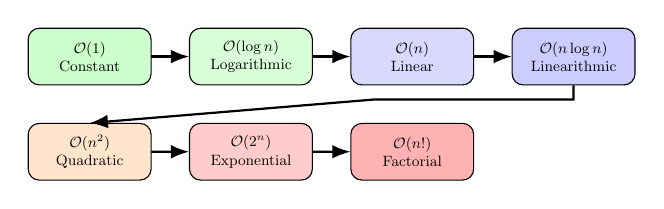
\begin{tikzpicture}[
            scale=0.6,
            transform shape,
            complexity/.style={draw, rounded corners, minimum width=2.6cm, minimum height=1.2cm, align=center, font=\small, fill=gray!10},
            arrow/.style={-{Latex}, thick},
            node distance=0.8cm and 0.8cm
        ]
    
            % First row
            \node[complexity, fill=green!20] (const) {$\mathcal{O}(1)$\\Constant};
            \node[complexity, right=of const, fill=green!15] (log) {$\mathcal{O}(\log n)$\\Logarithmic};
            \node[complexity, right=of log, fill=blue!15] (linear) {$\mathcal{O}(n)$\\Linear};
            \node[complexity, right=of linear, fill=blue!20] (nlogn) {$\mathcal{O}(n \log n)$\\Linearithmic};
        
            % Second row
            \node[complexity, below=of const, fill=orange!20] (quad) {$\mathcal{O}(n^2)$\\Quadratic};
            \node[complexity, right=of quad, fill=red!20] (expo) {$\mathcal{O}(2^n)$\\Exponential};
            \node[complexity, right=of expo, fill=red!30] (factorial) {$\mathcal{O}(n!)$\\Factorial};
        
            % Arrows row 1
            \draw[arrow] (const) -- (log);
            \draw[arrow] (log) -- (linear);
            \draw[arrow] (linear) -- (nlogn);
        
            % Arrow to second row
            \draw[arrow] (nlogn.south) -- ++(0,-0.3) -- ++(-4.2,0) -- (quad.north);
        
            % Arrows row 2
            \draw[arrow] (quad) -- (expo);
            \draw[arrow] (expo) -- (factorial);
    
        \end{tikzpicture}
    \end{center}

    \subsection*{Ackermann-Funktion}
    Ist definiert als:
    \[
    A(m, n) =
    \begin{cases}
        n + 1 & \text{für } m = 0 \\
        A(m - 1, 1) & \text{für } m > 0 \text{ \& } n = 0 \\
        A(m - 1, A(m, n - 1)) & \text{für } m > 0 \text{ \& } n > 0
    \end{cases}
    \]
    Die Ackermann-Funktion wächst sehr schnell und ist nicht in polynomieller Zeit berechenbar. Sie ist ein Beispiel für eine rekursive Funktion, die nicht primitiv rekursiv ist.
\end{minipage}

\begin{minipage}[t]{0.45\textwidth}
    \subsection*{Primitiv rekursive Funktionen}
    Eine Funktion ist \textbf{primitiv rekursiv}, wenn sie durch endliche Rekursion und Schleifen definiert ist. Beispiele sind Addition, Multiplikation.

    \subsection*{Rekursive Funktionen}
    Eine Funktion ist \textbf{rekursiv}, wenn sie durch eine Turingmaschine berechnet werden kann. Alle primitiven rekursiven Funktionen sind rekursiv, aber nicht alle rekursiven Funktionen sind primitiv rekursiv.

    \subsection*{Regeln}
    \begin{itemize}
        \item \textbf{Entscheidbarkeit}: Wenn $A$ entscheidbar ist, dann ist auch $A \cup B$ entscheidbar für jede Sprache $B$. (Gilt auch für semi-entscheidbare Sprachen.)
        \item \textbf{Semi-Entscheidbarkeit}: Wenn $A$ semi-entscheidbar ist, dann ist $\overline{A}$ nicht notwendigerweise semi-entscheidbar.
        \item \textbf{Reduktion}: Wenn $A \preceq B$ und $B$ entscheidbar ist, dann ist auch $A$ entscheidbar.
        \item \textbf{Komplement}: Wenn $A$ entscheidbar ist, dann ist auch das Komplement $\overline{A}$ entscheidbar.
        \item \textbf{Vereinigung und Schnittmenge}: Wenn $A$ und $B$ entscheidbar sind, dann sind auch $A \cup B$ und $A \cap B$ entscheidbar.
        \item \textbf{Submenge und Supermenge}: Wenn $A$ und $B$ entscheidbar sind, dann ist auch $A \subseteq B$ entscheidbar.
    \end{itemize}
\end{minipage}
\hfill
\begin{minipage}[t]{0.45\textwidth}
    \subsection*{Definitionen}
    \begin{itemize}
        \item \textbf{Schnittmenge}: $A \cap B = \{x | x \in A \text{ und } x \in B\}$
        \item \textbf{Vereinigung}: $A \cup B = \{x | x \in A \text{ oder } x \in B\}$
        \item \textbf{Submenge}: $A \subseteq B$ bedeutet, dass jedes Element von $A$ auch in $B$ enthalten ist.
        \item \textbf{Supermenge}: $A \supseteq B$ bedeutet, dass jedes Element von $B$ auch in $A$ enthalten ist.
        \item \textbf{Differenz}: $A \setminus B = \{x | x \in A \text{ und } x \notin B\}$
        \item \textbf{Komplement}: $\overline{A} = \{x | x \notin A\}$
        \item \textbf{Länge eines Wortes}: $|w|$ ist die Anzahl der Symbole in $w$.
        \item \textbf{Vorkommen eines Symbols}: $|w|_a$ ist die Anzahl der Vorkommen des Symbols $a$ in $w$.
        \item \textbf{Kleenesche Hülle}: $\Sigma^*$ ist die Menge aller endlichen Wörter über dem Alphabet $\Sigma$, einschließlich des leeren Wortes $\varepsilon$.
        \item \textbf{Kleenesche Plus}: $\Sigma^+$ ist die Menge aller endlichen Wörter über dem Alphabet $\Sigma$, ohne das leere Wort..
        \item \textbf{Konkatination}: Wenn $L_1$ und $L_2$ Sprachen sind, dann ist $L_1 L_2 = \{xy | x \in L_1 \text{ und } y \in L_2\}$ die Sprache, die aus der Verkettung aller Wörter von $L_1$ mit allen Wörtern von $L_2$ besteht.
    \end{itemize}
\end{minipage}
\end{document}